\documentclass[10pt]{article}

\usepackage[a4paper,top=15mm,bottom=16mm,left=16mm,right=16mm]{geometry}
\usepackage[T1]{fontenc}
\usepackage[utf8]{inputenc}
\usepackage[default]{sourcesanspro}
\usepackage{newtxmath}
\usepackage{microtype}
\usepackage{amsmath}
\usepackage{booktabs,tabularx,array,multirow}
\usepackage{ragged2e}
\usepackage{float}
\usepackage{xcolor}
\usepackage{tikz}
\usetikzlibrary{arrows.meta,positioning,calc}
\usepackage[most]{tcolorbox}
\usepackage{enumitem}
\usepackage{fancyhdr}
\usepackage{titlesec}
\usepackage{caption}
\usepackage[hidelinks]{hyperref}

\definecolor{Ink}{HTML}{102A43}
\definecolor{Navy}{HTML}{16324F}
\definecolor{Blue}{HTML}{1B6CA8}
\definecolor{Teal}{HTML}{168C82}
\definecolor{Green}{HTML}{268A64}
\definecolor{Gold}{HTML}{D18B28}
\definecolor{Red}{HTML}{B04444}
\definecolor{Slate}{HTML}{526777}
\definecolor{Mist}{HTML}{EEF4F7}
\definecolor{PaleBlue}{HTML}{E7F1F8}
\definecolor{PaleTeal}{HTML}{E7F5F3}
\definecolor{PaleGold}{HTML}{FBF3E4}
\definecolor{PaleRed}{HTML}{FAECEC}
\definecolor{Line}{HTML}{CCD9E2}

\hypersetup{
  colorlinks=true,
  linkcolor=Blue,
  urlcolor=Blue,
  citecolor=Blue,
  pdftitle={The Anatomy of a Polymarket Price},
  pdfauthor={Chronos Research Project}
}

\pagestyle{fancy}
\fancyhf{}
\fancyhead[L]{\footnotesize\color{Slate}\textbf{CHRONOS} \; RESEARCH WHITE PAPER 01}
\fancyhead[R]{\footnotesize\color{Slate}18 AUGUST 2026}
\fancyfoot[L]{\footnotesize\color{Slate}Prediction-market dynamics, validation, and limits}
\fancyfoot[R]{\footnotesize\color{Slate}\thepage}
\renewcommand{\headrulewidth}{0.35pt}
\renewcommand{\footrulewidth}{0pt}

\titleformat{\section}{\fontsize{17}{20}\selectfont\bfseries\color{Ink}}{}{0pt}{}
\titleformat{\subsection}{\fontsize{12}{14}\selectfont\bfseries\color{Blue}}{}{0pt}{}
\titleformat{\subsubsection}{\normalsize\bfseries\color{Ink}}{}{0pt}{}
\titlespacing*{\section}{0pt}{6pt}{5pt}
\titlespacing*{\subsection}{0pt}{6pt}{2pt}
\titlespacing*{\subsubsection}{0pt}{4pt}{1pt}

\setlength{\parindent}{0pt}
\setlength{\parskip}{4pt}
\setlength{\tabcolsep}{4.5pt}
\renewcommand{\arraystretch}{1.12}
\setlist[itemize]{leftmargin=5mm,itemsep=2pt,topsep=2pt}
\setlist[enumerate]{leftmargin=6mm,itemsep=2pt,topsep=2pt}
\captionsetup{font=small,labelfont=bf,skip=3pt}

\newtcolorbox{keybox}[1][]{
  enhanced,colback=PaleBlue,colframe=Blue,boxrule=0.6pt,arc=1.2mm,
  left=3mm,right=3mm,top=2.3mm,bottom=2.3mm,#1}
\newtcolorbox{warningbox}[1][]{
  enhanced,colback=PaleGold,colframe=Gold,boxrule=0.6pt,arc=1.2mm,
  left=3mm,right=3mm,top=2.3mm,bottom=2.3mm,#1}
\newtcolorbox{negativebox}[1][]{
  enhanced,colback=PaleRed,colframe=Red,boxrule=0.6pt,arc=1.2mm,
  left=3mm,right=3mm,top=2.3mm,bottom=2.3mm,#1}
\newtcolorbox{plainbox}[1][]{
  enhanced,colback=white,colframe=Line,boxrule=0.5pt,arc=1.2mm,
  left=3mm,right=3mm,top=2.3mm,bottom=2.3mm,before upper=\RaggedRight,#1}

\newcommand{\metriccard}[3]{%
\begin{minipage}[t]{0.238\linewidth}
\begin{tcolorbox}[enhanced,colback=white,colframe=Line,boxrule=0.6pt,arc=1.2mm,
height=29mm,valign=center,left=2mm,right=2mm,top=1mm,bottom=1mm]
\centering{\fontsize{19}{20}\selectfont\bfseries\color{Navy}#1}\par
{\small\bfseries\color{Ink}#2}\par
{\scriptsize\color{Slate}#3}
\end{tcolorbox}
\end{minipage}}

\newcommand{\term}[1]{\textbf{\color{Ink}#1}}
\newcommand{\good}{\textcolor{Green}{\textbf{PASS}}}
\newcommand{\fail}{\textcolor{Red}{\textbf{FAIL}}}
\newcommand{\pp}{percentage points}
\newcolumntype{Y}{>{\RaggedRight\arraybackslash}X}

\begin{document}

% =============================================================================
% PAGE 1 - COVER AND EXECUTIVE SUMMARY
% =============================================================================
\thispagestyle{fancy}
\begin{tcolorbox}[enhanced,colback=Navy,colframe=Navy,boxrule=0pt,arc=0mm,
left=7mm,right=7mm,top=8mm,bottom=8mm]
{\small\bfseries\color{white!72}CHRONOS RESEARCH PROJECT \hfill WORKING PAPER 01}\par
\vspace{8mm}
{\fontsize{30}{33}\selectfont\bfseries\color{white}The Anatomy of a\\Polymarket Price}\par
\vspace{3mm}
{\fontsize{16}{19}\selectfont\color{white!88}
Why prediction-market probabilities move in sticky jumps, not smooth diffusion}\par
\vspace{8mm}
{\small\color{white!70}A mathematical and machine-learning study of 803,862 hourly observations}\par
\end{tcolorbox}

\vspace{4mm}
\metriccard{62.4\%}{unchanged}{interior hourly samples}
\hfill
\metriccard{157.1}{kurtosis}{Gaussian benchmark: 3}
\hfill
\metriccard{112/113}{event comparisons}{full model beat state-only}
\hfill
\metriccard{0}{trade-ready signals}{after validation and costs}

\section*{The answer in one paragraph}

Polymarket probabilities do not move like a stock price following a smooth random walk. Most
recorded hours show no change at all. When the probability does move, the change is often abrupt,
its size depends on recent movement, and its direction is more likely to reverse than to continue.
Most importantly, a market that has been quiet for a long time is much less likely to update in the
next hour than a market that has just moved. A model that treats these as three separate questions
--- \emph{will it move, in which direction, and by how much?} --- fits later data materially better
than a bounded Gaussian diffusion. The finding is statistically useful, but it is not yet a
trading strategy: the strongest model predicts activity, not profitable direction.

\begin{minipage}[t]{0.315\linewidth}
\begin{plainbox}[height=51mm]
{\large\bfseries\color{Blue}What we studied}\par
Recorded YES probabilities from resolved Polymarket contracts, grouped by event and ordered in
time. A second cohort and official five-minute data were used to challenge the first result.
\end{plainbox}
\end{minipage}\hfill
\begin{minipage}[t]{0.315\linewidth}
\begin{plainbox}[height=51mm]
{\large\bfseries\color{Teal}What we found}\par
A jump process that explicitly allows no change, and remembers inactivity and recent movements,
describes the recorded data substantially better than smooth diffusion.
\end{plainbox}
\end{minipage}\hfill
\begin{minipage}[t]{0.315\linewidth}
\begin{plainbox}[height=51mm]
{\large\bfseries\color{Gold}What we did not find}\par
No protected, executable trading edge. Apparent flow and external-data signals weakened or became
negative after direction, fees, liquidity, and temporal controls.
\end{plainbox}
\end{minipage}

\vfill
{\footnotesize\color{Slate}\textbf{Status.} Development evidence, unchanged later-cohort replay,
and one retained protected negative. Independent research; not affiliated with Polymarket. Not
investment advice.}

\newpage

% =============================================================================
% PAGE 2 - OBJECT OF STUDY
% =============================================================================
\section*{1. What exactly is a Polymarket price?}

Suppose a contract asks: \emph{``Will Candidate A win the election?''} A YES share pays \$1 if the
answer is yes and \$0 if the answer is no. If a YES share trades around \$0.65, people often say
that the market assigns a 65\% probability to the event.

That interpretation can be useful, but it is not automatic. The displayed number is produced by
orders, trades, market rules, and a data feed. It may differ from the probability in traders'
heads, from the best price available for a new order, and from the true chance that the event will
happen. Prediction-market theory makes those distinctions explicit \cite{wolfers2004,manski2006}.

\begin{center}
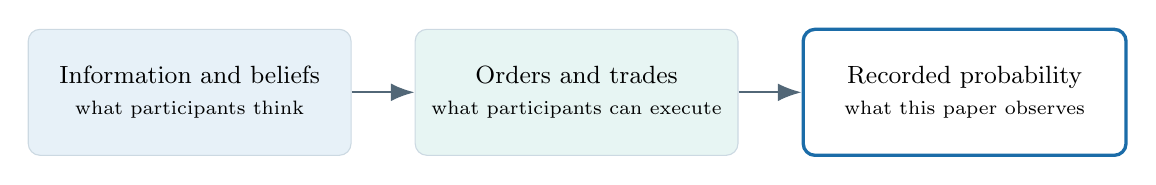
\begin{tikzpicture}[node distance=8mm, every node/.style={font=\small}]
\node[draw=Line,fill=PaleBlue,rounded corners=1.5mm,minimum width=41mm,minimum height=16mm,align=center] (belief) {Information and beliefs\\\scriptsize what participants think};
\node[draw=Line,fill=PaleTeal,rounded corners=1.5mm,minimum width=41mm,minimum height=16mm,align=center,right=of belief] (market) {Orders and trades\\\scriptsize what participants can execute};
\node[draw=Blue,fill=white,very thick,rounded corners=1.5mm,minimum width=41mm,minimum height=16mm,align=center,right=of market] (sample) {Recorded probability\\\scriptsize what this paper observes};
\draw[-{Latex[length=3mm]},thick,color=Slate] (belief) -- (market);
\draw[-{Latex[length=3mm]},thick,color=Slate] (market) -- (sample);
\end{tikzpicture}
\end{center}

\begin{keybox}
\textbf{The paper studies the final box.} It does not assume that a recorded probability is the
true probability, an executable quote, or a direct measurement of collective belief. Those are
separate empirical questions.
\end{keybox}

\subsection*{Why ordinary stock-price intuition is incomplete}

An equity can, in principle, keep rising for decades. A binary contract cannot. Its price lives
between 0 and 1 and eventually resolves to exactly one of those values. News may arrive in bursts,
and long periods may pass with no meaningful update. There is also no continuously traded
underlying asset that lets an investor replicate the contract in the Black--Scholes sense.

This changes the mathematical starting point:

\begin{tabularx}{\linewidth}{>{\bfseries\color{Ink}\RaggedRight\arraybackslash}p{0.24\linewidth}YY}
\toprule
Question & Conventional default & Prediction-market complication \\
\midrule
State space & Often unbounded or positive & Probability is bounded in $[0,1]$ \\
End point & Asset continues trading & Contract resolves to 0 or 1 \\
Information clock & Often approximated as continuous & News and participation arrive irregularly \\
Replication & Underlying asset may be traded & Usually no replicating underlying \\
Observation & Trade or quote has a defined role & Sample may mix feed, quote, and trade mechanics \\
\bottomrule
\end{tabularx}

\subsection*{The two questions}

\begin{enumerate}
  \item Which parts of financial time-series theory remain useful once these structural differences are respected?
  \item Which stochastic-process family best describes and predicts the recorded Polymarket probability series?
\end{enumerate}

The first paper deliberately stops before claiming a strategy. A process can be predictable in
\emph{timing} or \emph{volatility} while remaining useless for predicting profitable direction.

\newpage

% =============================================================================
% PAGE 3 - DATA AND DESIGN
% =============================================================================
\section*{2. Data designed to survive skeptical review}

The main analysis uses 562 resolved markets from 157 event groups. It contains 803,862 recorded
hourly probabilities. A later cohort contributes 29 new event groups, and ten preselected markets
are checked against independently acquired official five-minute price histories.

\begin{center}
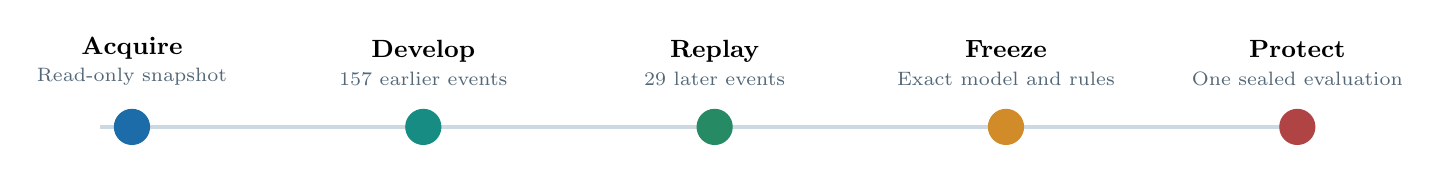
\begin{tikzpicture}[x=1mm,y=1mm,font=\small]
\draw[line width=1.2pt,color=Line] (5,0) -- (158,0);
\foreach \x/\title/\sub/\col in {
  9/Acquire/Read-only snapshot/Blue,
  46/Develop/157 earlier events/Teal,
  83/Replay/29 later events/Green,
  120/Freeze/Exact model and rules/Gold,
  157/Protect/One sealed evaluation/Red}
{
  \fill[\col] (\x,0) circle (2.3);
  \node[align=center,anchor=south] at (\x,4) {\bfseries\title\\[-1pt]\scriptsize\color{Slate}\sub};
}
\end{tikzpicture}
\end{center}

\begin{tabularx}{\linewidth}{YrrrY}
\toprule
Evidence set & Events & Markets & Observations & Purpose \\
\midrule
Main development cohort & 157 & 562 & 803,862 & Description and chronological model fitting \\
Later cohort & 29 & 147 & 42,549$^{a}$ & Replay the frozen law without refitting \\
Official five-minute panel & 10 & 10 & 19,258 & Test whether hourly sampling creates the result \\
Formal arrival schedule & 111 & -- & 231 decisions & Governed model evaluation \\
\bottomrule
\end{tabularx}
{\scriptsize\color{Slate}$^{a}$Observations used in the later process-signature replay. Exact
corpus identities appear in Appendix B.}

\subsection*{Four rules prevent an attractive story from becoming a false result}

\begin{minipage}[t]{0.49\linewidth}
\begin{plainbox}[height=33mm]
\term{1. Time only moves forward}\par
A feature may use only information already available at the forecast time. Training events must
occur before test events.
\end{plainbox}
\end{minipage}\hfill
\begin{minipage}[t]{0.49\linewidth}
\begin{plainbox}[height=33mm]
\term{2. Events, not rows, carry the uncertainty}\par
Markets tied to one real-world event are dependent. The analysis gives each event equal total
weight and keeps whole events together.
\end{plainbox}
\end{minipage}

\begin{minipage}[t]{0.49\linewidth}
\begin{plainbox}[height=33mm]
\term{3. Later evidence must be genuinely later}\par
The strongest law is fitted once, frozen, and applied unchanged to a later cohort. This tests
transfer rather than another round of tuning.
\end{plainbox}
\end{minipage}\hfill
\begin{minipage}[t]{0.49\linewidth}
\begin{plainbox}[height=33mm]
\term{4. Failure is part of the system}\par
A model that cannot legally produce a forecast has failed that decision. Missing forecasts cannot
be removed after their outcomes are seen.
\end{plainbox}
\end{minipage}

\subsection*{Three clocks are kept separate}

The analysis distinguishes the next recorded sample, the actual elapsed UTC time, and the time
remaining until market close. Headline one-hour changes require an elapsed gap between 45 and 75
minutes. A 24-hour variance calculation is accepted only when the elapsed time is close to 24
hours. This avoids treating irregularly spaced observations as if they were equally spaced.

\begin{warningbox}
\textbf{Why this matters.} Randomly shuffling individual rows would let nearly identical contracts
from the same event appear in both training and test data. It would also let future market regimes
inform the past. Both shortcuts can make weak models look impressive.
\end{warningbox}

\newpage

% =============================================================================
% PAGE 4 - EMPIRICAL SHAPE
% =============================================================================
\section*{3. What the probability paths actually look like}

The series is dominated by inactivity punctuated by abrupt updates. That is not a metaphor: among
regular interior hourly observations, 62.40\% are exactly unchanged. The distribution of changes
also has far more extreme observations than a Gaussian law: its raw kurtosis is 157.10, compared
with 3 for a Gaussian distribution.

\subsection*{The longer a market stays quiet, the less likely it is to move next}

\begin{center}
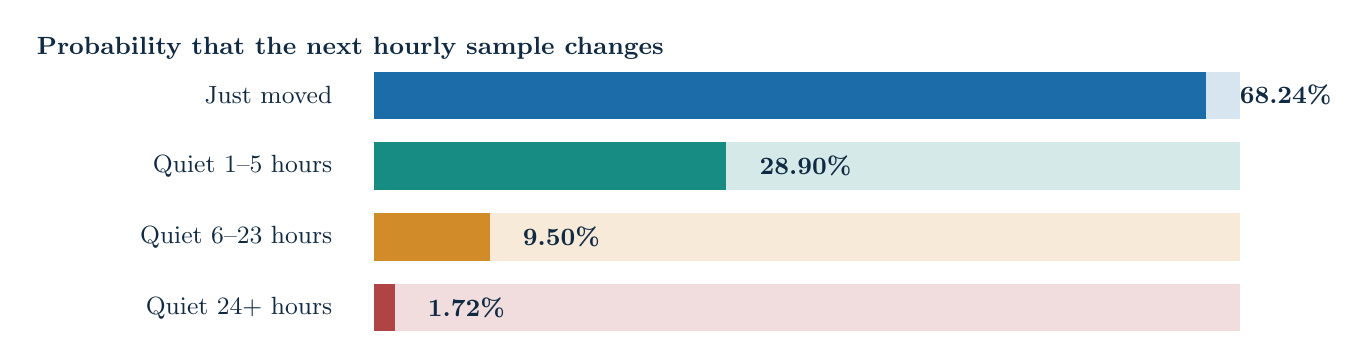
\begin{tikzpicture}[x=1mm,y=1mm,font=\small]
\node[anchor=west,font=\small\bfseries,color=Ink] at (0,36) {Probability that the next hourly sample changes};
\foreach \label/\val/\y/\col in {Just moved/68.24/27/Blue,Quiet 1--5 hours/28.90/18/Teal,Quiet 6--23 hours/9.50/9/Gold,Quiet 24+ hours/1.72/0/Red}{
  \node[anchor=east,color=Ink] at (40,\y+3) {\label};
  \fill[\col!18] (44,\y) rectangle (154,\y+6);
  \fill[\col] (44,\y) rectangle ({44+1.55*\val},\y+6);
  \node[anchor=west,font=\small\bfseries,color=Ink] at ({47+1.55*\val},\y+3) {\val\%};
}
\end{tikzpicture}
\end{center}

A market that has already been unchanged for at least 24 hours moves in the next recorded hour
only 1.72\% of the time. A market that just moved changes again 68.24\% of the time. A constant-rate
Poisson clock cannot explain a difference of this size. In statistical language, the arrival
hazard has memory; in plain language, activity clusters.

\subsection*{Five signatures contradict smooth diffusion}

\begin{tabularx}{\linewidth}{>{\bfseries\color{Ink}\RaggedRight\arraybackslash}p{0.24\linewidth}>{\RaggedRight\arraybackslash}p{0.20\linewidth}Y}
\toprule
Observed property & Main estimate & Why it matters \\
\midrule
Exact zero changes & 62.40\% interior hourly & A continuous Gaussian law has no point mass at zero \\
Extreme tails & Kurtosis 157.10 & Large updates occur far more often than Gaussian scaling suggests \\
Sub-diffusive scaling & 24h ratio 0.235 pooled & Variance does not grow linearly with clock time \\
Sign reversal & 62.21\% of adjacent nonzero moves & Recorded directions are not independent \\
Boundary persistence & 98.99\% low; 97.07\% high & Contracts behave differently near 0 and 1 \\
\bottomrule
\end{tabularx}

\subsection*{Could the data feed be creating the pattern?}

That is the most important rival explanation. The five-minute panel therefore repeats the test on
an independently acquired official source. The pattern becomes stronger, not weaker: 78.00\% zero
changes, kurtosis 203.64, reversal 67.87\%, and a 24-hour variance ratio of 0.067. Of 1,580 hourly
samples that can be aligned to the official history within ten minutes, 99.49\% match exactly.

The test does \emph{not} prove that latent beliefs jump. It shows that coarse hourly sampling alone
does not manufacture the observed structure on this panel. The registered series may still mix
economic inactivity, stale quotes, rounding, bid/ask effects, and the way the venue publishes its
history.

\begin{keybox}
\textbf{Finding 1.} The recorded probability process is sticky and bursty. A useful model needs an
explicit probability of no change, not merely a small continuous volatility.
\end{keybox}

\newpage

% =============================================================================
% PAGE 5 - MODEL
% =============================================================================
\section*{4. A model built around how the market updates}

Rather than force every hour into one return distribution, the leading model asks three questions
in sequence:

\begin{center}
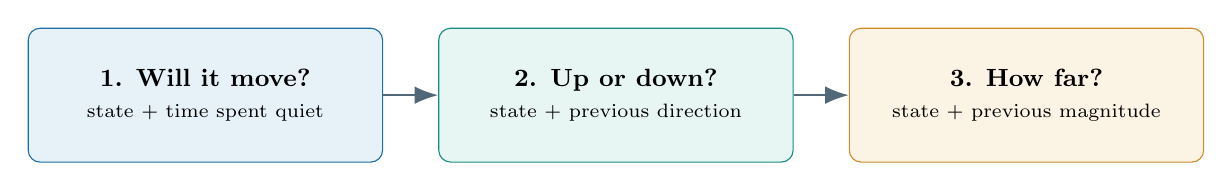
\begin{tikzpicture}[node distance=7mm,font=\small]
\node[draw=Blue,fill=PaleBlue,rounded corners=1.5mm,minimum width=45mm,minimum height=17mm,align=center] (move) {\bfseries 1. Will it move?\\\scriptsize state + time spent quiet};
\node[draw=Teal,fill=PaleTeal,rounded corners=1.5mm,minimum width=45mm,minimum height=17mm,align=center,right=of move] (sign) {\bfseries 2. Up or down?\\\scriptsize state + previous direction};
\node[draw=Gold,fill=PaleGold,rounded corners=1.5mm,minimum width=45mm,minimum height=17mm,align=center,right=of sign] (size) {\bfseries 3. How far?\\\scriptsize state + previous magnitude};
\draw[-{Latex[length=3mm]},thick,color=Slate] (move) -- (sign);
\draw[-{Latex[length=3mm]},thick,color=Slate] (sign) -- (size);
\end{tikzpicture}
\end{center}

Let $P_t$ be the recorded YES probability. The model first assigns probability $q_t$ to a nonzero
change. Conditional on moving, it assigns probability $s_t$ to an upward move and models the log
size of the change with a Gaussian distribution:
\begin{align*}
\Pr(\Delta P_{t+1}=0\mid\mathcal F_t)&=1-q_t,\\
\Pr(\Delta P_{t+1}>0\mid\Delta P_{t+1}\neq0,\mathcal F_t)&=s_t,\\
\log|\Delta P_{t+1}|\mid\Delta P_{t+1}\neq0,\mathcal F_t&\sim
\mathcal N(\mu_t,\tau_t^2).
\end{align*}
The information set $\mathcal F_t$ contains only legally available features: current probability,
time to close, quiet duration, recent inactivity, previous nonzero direction, and previous nonzero
size. Appendix A gives the exact scoring rule.

\subsection*{The full model wins because each layer contributes}

The models are judged by negative log likelihood (NLL): how much probability they assigned to what
actually happened. Lower is better. Event-level NLL first averages within each event and then gives
every event equal weight.

\begin{center}
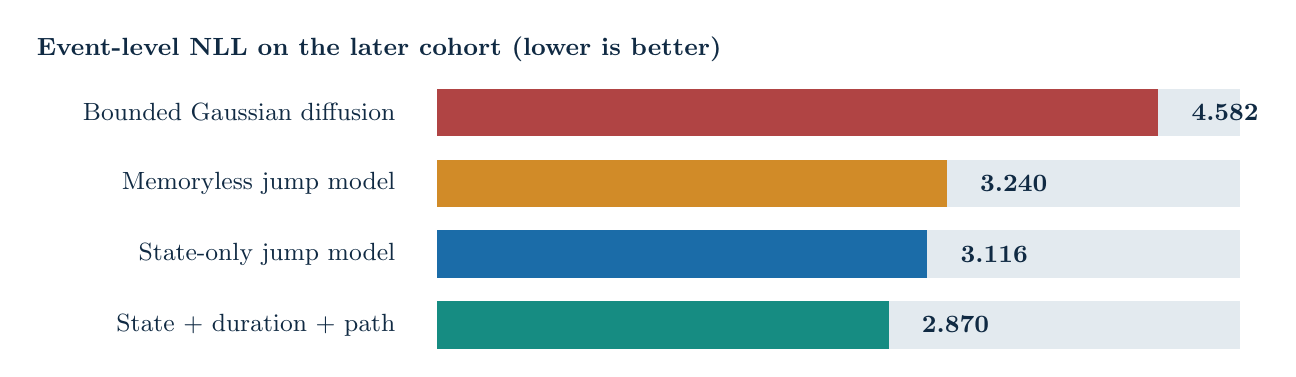
\begin{tikzpicture}[x=1mm,y=1mm,font=\small]
\node[anchor=west,font=\small\bfseries,color=Ink] at (0,38) {Event-level NLL on the later cohort (lower is better)};
\foreach \label/\val/\y/\col in {Bounded Gaussian diffusion/4.582/27/Red,Memoryless jump model/3.240/18/Gold,State-only jump model/3.116/9/Blue,State + duration + path/2.870/0/Teal}{
  \node[anchor=east,color=Ink] at (48,\y+3) {\label};
  \fill[Line!55] (52,\y) rectangle (154,\y+6);
  \fill[\col] (52,\y) rectangle ({52+20*\val},\y+6);
  \node[anchor=west,font=\small\bfseries,color=Ink] at ({55+20*\val},\y+3) {\val};
}
\end{tikzpicture}
\end{center}

In the development cohort, the full model improves event-level NLL by 7.74\% over the state-only
jump model and wins 112 of 113 event comparisons. The model is then frozen and applied, without
refitting, to the later cohort. It improves by 7.88\% and wins all 27 eligible events against both
the state-only model and diffusion.

Absolute scores are worse in the later cohort. That matters: the mathematical structure transfers,
but the parameter levels change. The result supports a stable \emph{family} of models with
regime-dependent parameters, not one universal coefficient vector.

\begin{keybox}
\textbf{Finding 2.} A bounded, zero-inflated marked-jump model with duration and path information
describes later Polymarket data better than smooth diffusion. The result transfers without
refitting, although its exact calibration changes across cohorts.
\end{keybox}

\newpage

% =============================================================================
% PAGE 6 - PREDICTION AND PROTECTED NEGATIVE
% =============================================================================
\section*{5. Strong predictive component, rejected protected system}

The most reliable part of the model is the first question: \emph{will the recorded probability
change in the next hour?} A regularized logistic model uses current state, time to close, the logarithm of the quiet
run, and the fraction of unchanged observations during the previous 24 hours.

\begin{minipage}[t]{0.48\linewidth}
\begin{plainbox}[height=44mm]
{\small\bfseries\color{Slate}LATER COHORT: EVENT-LEVEL BRIER SCORE}\par
\vspace{2mm}
{\fontsize{22}{23}\selectfont\bfseries\color{Red}0.261}\;{\large\color{Slate}$\rightarrow$}\;
{\fontsize{22}{23}\selectfont\bfseries\color{Teal}0.174}\par
{\small State only \hfill + inactivity}\par
\vspace{1mm}
{\small\color{Ink}\textbf{33.38\% improvement}; 27 wins in 27 eligible events.}
\end{plainbox}
\end{minipage}\hfill
\begin{minipage}[t]{0.48\linewidth}
\begin{plainbox}[height=44mm]
{\small\bfseries\color{Slate}WHAT A BRIER SCORE MEANS}\par
\vspace{2mm}
It is the average squared error of a probability forecast. Zero is perfect. The model's mean
forecast was 41.29\%; the next hour changed 45.34\% of the time. The absolute calibration gap was
4.05 \pp.
\end{plainbox}
\end{minipage}

This is meaningful predictive evidence. It is also narrower than it first appears. The model says
when a recorded update is likely; it does not say whether the update will be up or down, whether an
order can be filled, or whether a trade will earn more than its costs.

\subsection*{Why the final system was rejected}

After development, an exact version of the continuous inactivity model was frozen: source code,
features, training window, decision schedule, metrics, and failure rules. It was then evaluated
once on protected data.

\begin{center}

\begin{tikzpicture}[x=1mm,y=1mm,font=\small]
\node[anchor=west,font=\small\bfseries,color=Ink] at (0,18) {Declared protected decisions};
\fill[PaleTeal] (0,5) rectangle (160,13);
\fill[Teal] (0,5) rectangle (104,13);
\fill[Red] (104,5) rectangle (160,13);
\node[color=white,font=\small\bfseries] at (52,9) {65 completed};
\node[color=white,font=\small\bfseries] at (132,9) {35 failed};
\end{tikzpicture}
\end{center}

On the 65 completed decisions, Brier score was 0.189 and mean absolute error was 0.394, both inside
the predeclared limits. But the system was required to complete at least 95 of 100 decisions. It
completed only 65. Thirty-four decisions lacked the fixed legal training history and one lacked a
legally available outcome. Error concentration also narrowly missed its limit.

\begin{negativebox}
\textbf{Protected decision: rejected.} Coverage was 65\% against a required 95\%; failure rate was
35\% against a maximum 5\%. The completed rows cannot be presented as a successful model because
the missing decisions may be systematically harder than the completed ones.
\end{negativebox}

This distinction is central. A model is not merely an equation evaluated on convenient rows. It is
the complete decision process, including whether the required history exists and whether it can
produce forecasts on schedule. The protected failure does not erase the earlier evidence that
inactivity matters. It prevents that evidence from being promoted into a broader validated claim.

\begin{keybox}
\textbf{Finding 3.} Quiet duration is a powerful predictor of recorded update timing. The exact
protected implementation is nevertheless rejected because it failed too many declared decisions.
\end{keybox}

\newpage

% =============================================================================
% PAGE 7 - INTERPRETATION
% =============================================================================
\section*{6. What this changes - and what comes next}

The evidence supports a different default model for Polymarket research. Instead of beginning with
a smooth return process and adding occasional anomalies, begin with an event-linked process that
can remain unchanged, update in clusters, and terminate at a binary boundary.

\begin{tabularx}{\linewidth}{>{\bfseries\color{Ink}\RaggedRight\arraybackslash}p{0.27\linewidth}>{\RaggedRight\arraybackslash}p{0.19\linewidth}Y}
\toprule
Financial idea & Verdict & Required modification \\
\midrule
Chronological validation & Transfers & Split and weight by real-world event, not individual rows \\
State-dependent volatility & Transfers & Respect probability bounds and terminal resolution \\
Duration and point-process models & Transfers strongly & Model time since the last update as part of the state \\
Heavy-tailed returns & Transfers conditionally & First separate zero changes and conditional size \\
Martingale reasoning & Useful benchmark & Distinguish sampled price, executable price, belief, and physical probability \\
Constant Brownian diffusion & Poor default & Add point mass, jumps, irregular information time, and boundaries \\
Black--Scholes replication & Does not transfer directly & No standard replicating underlying or complete market \\
\bottomrule
\end{tabularx}

\subsection*{Why this is not yet a trading paper}

The strongest result predicts movement timing. Directional ideas have been tested separately and
have not survived the full controls:

\begin{itemize}
  \item A raw 15-minute flow association near $-0.46$ fell to about $+0.04$ to $+0.05$ after
  transaction direction was handled correctly.
  \item In the Brazil election study, 31 poll releases produced 25 usable decisions and 17,570
  canonical fills. The broad 72-hour fade earned \$10.69 before costs and lost \$18.97 after
  conservative fees.
  \item Other event and internal-market rules were also rejected or remained descriptive because
  they lacked executable quotes, sufficient breadth, or protected confirmation.
\end{itemize}

These are useful results. They show why statistical association, price prediction, and tradable
edge are three different standards.

\subsection*{The next research programme}

\begin{enumerate}
  \item Use the inactivity hazard as an \emph{eligibility layer}: predict direction only when a
  movement is likely enough to make the forecast operationally relevant.
  \item Add time-legal external information --- including polls, macro releases, and prices from
  other prediction venues --- as predictors, not as presumed arbitrage.
  \item Evaluate direction and magnitude chronologically, then translate predictions into
  side-specific Polymarket orders with spread, fees, latency, depth, and abstention.
  \item Reserve a genuinely new protected cohort for any system that clears fixed development
  gates. The exposed protected schedule from this paper cannot be reused.
\end{enumerate}

\begin{tcolorbox}[enhanced,colback=Navy,colframe=Navy,boxrule=0pt,arc=1.5mm,
left=5mm,right=5mm,top=4mm,bottom=4mm]
{\large\bfseries\color{white}Bottom line}\par
{\color{white!90}Polymarket's recorded probabilities are best understood as a bounded,
state-dependent jump process with long quiet periods and clustered updates. That finding is broad,
reproducible, and mathematically useful. It is a foundation for better forecasting and simulation
--- not evidence that a profitable strategy has already been found.}
\end{tcolorbox}

\vfill
{\footnotesize\color{Slate}The appendix records the exact equations, corpus identities, robustness
checks, negative results, limitations, and references.}

\newpage
\appendix
\renewcommand{\thesection}{\Alph{section}}
\titleformat{\section}{\fontsize{15}{18}\selectfont\bfseries\color{Ink}}{Appendix \thesection}{0.65em}{}

% =============================================================================
% APPENDIX A-B
% =============================================================================
\section{Exact model and scoring definitions}

Let $P_t\in[0,1]$ be the registered YES probability and
$\Delta P_{t+1}=P_{t+1}-P_t$. The bounded Gaussian comparator is
\begin{equation}
\Delta P_{t+1}\mid\mathcal F_t\sim
\mathcal N\!\left(0,\sigma^2(c_t)P_t(1-P_t)\right),
\end{equation}
where $c_t$ is a fixed probability and time-to-close cell. The bounded factor shrinks local
variance near 0 and 1 but retains a continuous Gaussian increment law.

The full hurdle law is
\begin{align}
\Pr(\Delta P_{t+1}=0\mid\mathcal F_t)&=1-q(\mathcal F_t),\\
\Pr(\Delta P_{t+1}>0\mid\Delta P_{t+1}\neq0,\mathcal F_t)&=s(\mathcal F_t),\\
\log|\Delta P_{t+1}|\mid\Delta P_{t+1}\neq0,\mathcal F_t&\sim
\mathcal N(\mu(\mathcal F_t),\tau^2(\mathcal F_t)).
\end{align}
Arrival uses probability and quiet-duration cells; sign uses probability and previous nonzero sign;
magnitude uses probability and previous nonzero magnitude. Each cell shrinks toward the
event-equal global law with one event of prior weight.

For nonzero $x$, the model assigns probability to the same 0.001-wide interval for every family:
\begin{align}
&q(\mathcal F_t)\Pr(\operatorname{sign}x\mid\mathcal F_t)\times\\[-3pt]
&\left[\Phi\!\left(\frac{\log(|x|+\epsilon)-\mu}{\tau}\right)-
\Phi\!\left(\frac{\log(\max(10^{-6},|x|-\epsilon))-\mu}{\tau}\right)\right],
\end{align}
with $\epsilon=0.0005$. A zero receives point mass $1-q(\mathcal F_t)$. Negative log interval
probability is averaged by observation and separately by event.

The continuous arrival model predicts $Y_{t+1}=1[\Delta P_{t+1}\neq0]$:
\begin{equation}
\operatorname{logit}\Pr(Y_{t+1}=1\mid\mathcal F_t)=
\beta_0+\beta_p f(P_t)+\beta_T f(T_t)+\beta_q\log(1+Q_t)+\beta_z Z_{t,24},
\end{equation}
where $Q_t$ is the current quiet run and $Z_{t,24}$ is the previous-24-hour zero fraction. Its
Brier score is $n^{-1}\sum_i(\widehat q_i-Y_i)^2$.

\section{Data authority and corpus identity}

The opening 1,000-contract corpus contains 235 events and 1,180,437 observations. The successor
acquisition contains 1,509 contracts, 321 events, and 1,585,740 observations. Its content identity
is:
\begin{quote}\small\ttfamily
polymarket-corpus:184b83f7f8012da4ca9116c8b6bad2076570ad5f0bada95b22615ee2f5cceae8
\end{quote}
The successor partition contains 29 wholly fresh development events (147 markets), 227 embargoed
ancestor events (1,005 markets), and 65 protected events (357 markets). Data were acquired through
the read-only \texttt{human\_ro} role. Chronos retains source digests, selection, temporal
semantics, partitions, actual field accesses, worker outcomes, and result receipts.

\newpage

% =============================================================================
% APPENDIX C-D
% =============================================================================
\section{Complete numerical results}

\begin{table}[H]
\centering\small
\begin{tabularx}{\linewidth}{Yrrr}
\toprule
Model & Development observation NLL & Development event NLL & Later event NLL \\
\midrule
Bounded state-dependent Gaussian diffusion & 3.511 & 3.578 & 4.582 \\
Memoryless zero-inflated marked jump & 1.865 & 2.214 & 3.240 \\
State-conditioned zero-inflated marked jump & 1.782 & 2.104 & 3.116 \\
State + duration/path marked jump & \textbf{1.585} & \textbf{1.941} & \textbf{2.870} \\
\bottomrule
\end{tabularx}
\caption{Complete observation-law comparison. Lower NLL is better.}
\end{table}

\begin{table}[H]
\centering\small
\begin{tabular}{lrrl}
\toprule
Protected check & Result & Required & Decision \\
\midrule
Brier on completed rows & 0.189254 & $\leq0.200000$ & \good \\
MAE on completed rows & 0.394489 & $\leq0.400000$ & \good \\
Coverage & 0.650000 & $\geq0.950000$ & \fail \\
Failure rate & 0.350000 & $\leq0.050000$ & \fail \\
Maximum error concentration & 0.054852 & $\leq0.050000$ & \fail \\
\bottomrule
\end{tabular}
\caption{Single protected evaluation of the frozen continuous arrival system.}
\end{table}

\section{Representation and structural robustness}

\begin{table}[H]
\centering\small
\begin{tabular}{lrrrr}
\toprule
Fixed view & Increments & Zero rate & Kurtosis & Event-equal 24h ratio \\
\midrule
All probability rows & 781,388 & 69.73\% & 157.10 & 0.358 \\
Strict interior probability & 519,495 & 62.76\% & 103.19 & 0.376 \\
Strict interior log-odds & 519,495 & 62.76\% & 104.99 & 0.403 \\
More than 168 hours to close & 701,428 & 69.40\% & 151.06 & 0.338 \\
Zero to 168 hours to close & 79,960 & 72.54\% & 138.44 & 0.512 \\
\bottomrule
\end{tabular}
\caption{Boundary, coordinate, and maturity checks.}
\end{table}

\begin{table}[H]
\centering\small
\begin{tabular}{lrrrr}
\toprule
Whole-event stratum & Zero mass & Variance ratio & Reversal & Quiet ratio \\
\midrule
One-market events & 0.577 & 0.403 & 0.588 & 0.084 \\
At least five markets & 0.527 & 0.267 & 0.598 & 0.032 \\
Lifetime $\leq30$ days & 0.477 & 0.293 & 0.581 & 0.038 \\
Lifetime 31--180 days & 0.605 & 0.425 & 0.594 & 0.078 \\
Lifetime $>180$ days & 0.623 & 0.228 & 0.643 & 0.035 \\
Fewer than 500 points & 0.458 & 0.315 & 0.556 & 0.014 \\
500--1,999 points & 0.586 & 0.394 & 0.601 & 0.070 \\
At least 2,000 points & 0.631 & 0.248 & 0.635 & 0.053 \\
\bottomrule
\end{tabular}
\caption{Event-equal heterogeneity. Structural directions persist; parameter levels change.}
\end{table}

\newpage

% =============================================================================
% APPENDIX E-G
% =============================================================================
\section{Negative directional and external-data evidence}

\subsection*{Fill-semantics correction}
Polymarket's retained fill table is a per-party ledger. Counting maker and taker legs as separate
market trades duplicates economic activity and can invert direction. Canonical studies retain the
transaction-side record and convert YES and NO activity to a consistent YES-equivalent price and
taker direction. The raw 15-minute flow association near $-0.46$ fell to about $+0.04$ to $+0.05$
after this correction.

\subsection*{Brazil polling study}
Thirty-one national Lula/Fl\'avio runoff poll releases were reconstructed from immutable publication
history. They yielded 25 decisions and 17,570 canonical Polymarket fills. Features included latest
poll change, rolling-three median change, surprise against the previous five releases, and
same-pollster change. Follow and fade rules were tested at 0, 2, and 4 \pp\ thresholds over 24, 72,
and 168 hours. Every rule with at least five executable pairs was negative after conservative fees.
The broad 72-hour fade moved from \$10.69 gross to $-\$18.97$ net over seven trades.

\section{Claim ledger and limitations}

\begin{tabularx}{\linewidth}{>{\RaggedRight\arraybackslash}p{0.34\linewidth}>{\RaggedRight\arraybackslash}p{0.22\linewidth}Y}
\toprule
Claim & Status & Boundary \\
\midrule
Smooth constant-intensity diffusion describes registered samples & Rejected & Zero mass, tails, scaling, and duration dependence \\
State-duration/path jump law improves predictive density & Strong development + later replay & Not a protected finding; targets samples \\
Inactivity improves update prediction & Strong development + later replay & Exact protected system rejected \\
Boundaries alone explain stickiness & Rejected as sole cause & Interior and log-odds checks agree \\
Hourly sampling alone creates the signatures & Rejected on selected panel & Official five-minute source agrees \\
Sign reversal is executable mean reversion & Not established & Quotes, spread, fees, and latency absent \\
Chronos has found tradable alpha & No & Cost-aware directional ideas rejected \\
\bottomrule
\end{tabularx}

\begin{itemize}
  \item Registered samples are not identified as trades, quotes, midpoints, latent beliefs, or executable prices.
  \item The five-minute panel contains ten preselected markets; it is not a venue-wide quote study.
  \item Event grouping mitigates but cannot remove every dependence among related contracts.
  \item The diffusion comparator is intentionally simple and does not eliminate every latent continuous-time model with microstructure noise or endogenous sampling.
  \item One protected system was evaluated and rejected. Its exposed holdout cannot be reused.
  \item No result establishes causal information arrival, objective-probability equality, Sharpe ratio, or net profit after all execution costs.
\end{itemize}

\newpage
\section{References and reproducibility}
\begingroup\small
\renewcommand{\refname}{}
\vspace{-8mm}
\begin{thebibliography}{9}
\bibitem{bacry2013} Bacry, E., Delattre, S., Hoffmann, M., and Muzy, J.-F. (2013). Modelling microstructure noise with mutually exciting point processes. \emph{Quantitative Finance}, 13(1), 65--77.
\bibitem{brier1950} Brier, G. W. (1950). Verification of forecasts expressed in terms of probability. \emph{Monthly Weather Review}, 78(1), 1--3.
\bibitem{engle1998} Engle, R. F. and Russell, J. R. (1998). Autoregressive conditional duration. \emph{Econometrica}, 66(5), 1127--1162.
\bibitem{hawkes1971} Hawkes, A. G. (1971). Spectra of self-exciting and mutually exciting point processes. \emph{Biometrika}, 58(1), 83--90.
\bibitem{majumder2009} Majumder, S. R. et al. (2009). Price dynamics in political prediction markets. \emph{PNAS}, 106(3), 679--684.
\bibitem{manski2006} Manski, C. F. (2006). Interpreting the predictions of prediction markets. \emph{Economics Letters}, 91(3), 425--429.
\bibitem{prado2018} L\'opez de Prado, M. (2018). \emph{Advances in Financial Machine Learning}. Wiley.
\bibitem{wolfers2004} Wolfers, J. and Zitzewitz, E. (2004). Prediction markets. \emph{Journal of Economic Perspectives}, 18(2), 107--126.
\bibitem{wolfers2006} Wolfers, J. and Zitzewitz, E. (2006). Interpreting prediction market prices as probabilities. NBER Working Paper 12200.
\end{thebibliography}
\endgroup

Numerical claims map to content-addressed receipts in \texttt{paper/evidence-index.md}. Replay
commands and the non-rerunnable protected boundary are documented in
\texttt{paper/reproducibility.md}. The manuscript is a presentation layer; it cannot promote the
epistemic status of any result.

\vfill
{\footnotesize\color{Slate}Chronos Research Project. Working paper for scientific review. Not investment advice.}

\end{document}
